\section{Из чего состоит компьютер}\label{base:introduction:components}
\subsection{Общий обзор}\label{base:introduction:components:review}
Рассмотрим типичный персональный компьютер. В общем случае он состоит из устройства вывода изображения (монитор), большой шумящей коробки (системный блок) и разных устройств поменьше.
\begin{figure}[h!]
 \centering
 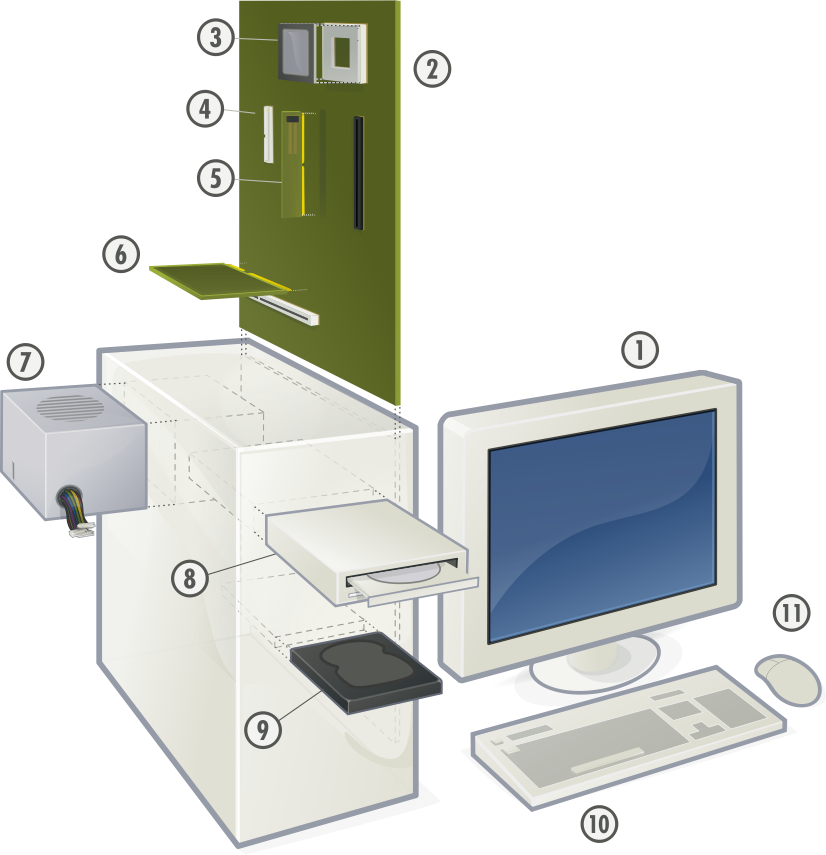
\includegraphics[width=0.5\textwidth]{base/Introduction/Computer.png}
 \label{Base:introduction:components:review:computerpic}
 \caption{Устройство персонального компьютера:}
 \footnotesize
 \begin{enumerate}
  \item монитор;
  \item материнская плата;
  \item процессор;
  \item порт ATA;
  \item оперативная память;
  \item карты расширений;
  \item блок питания;
  \item дисковод;
  \item жёсткий диск;
  \item клавиатура;
  \item компьютерная мышь;
 \end{enumerate}
\end{figure}

\subsection{Системный блок}\label{base:introduction:components:case}
Начнём наше знакомство с основного компонента настольного компьютера --- \emph{системного блока} (англ.~\emph{computer case} или \emph{computer chassis}). Сам по себе системный блок (по какой-то совершенно неясной причине иногда называемый <<процессором>>; наука пытается найти объяснение этому явлению) является корпусом, в котором располагаются все основные компоненты.
\begin{figure}[h!]
 \centering
 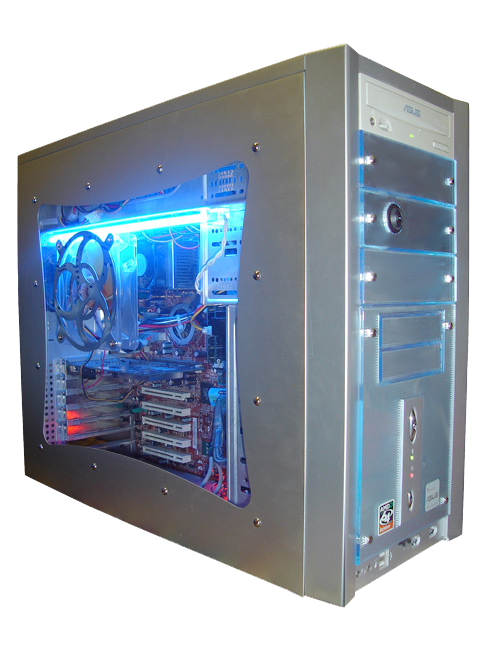
\includegraphics[width=0.5\textwidth]{base/Introduction/Case.png}
 \caption{Типичный системный блок}
 \label{base:introduction:components:case:typicalcasepic}
\end{figure}
\begin{figure}[h!]
 \centering
 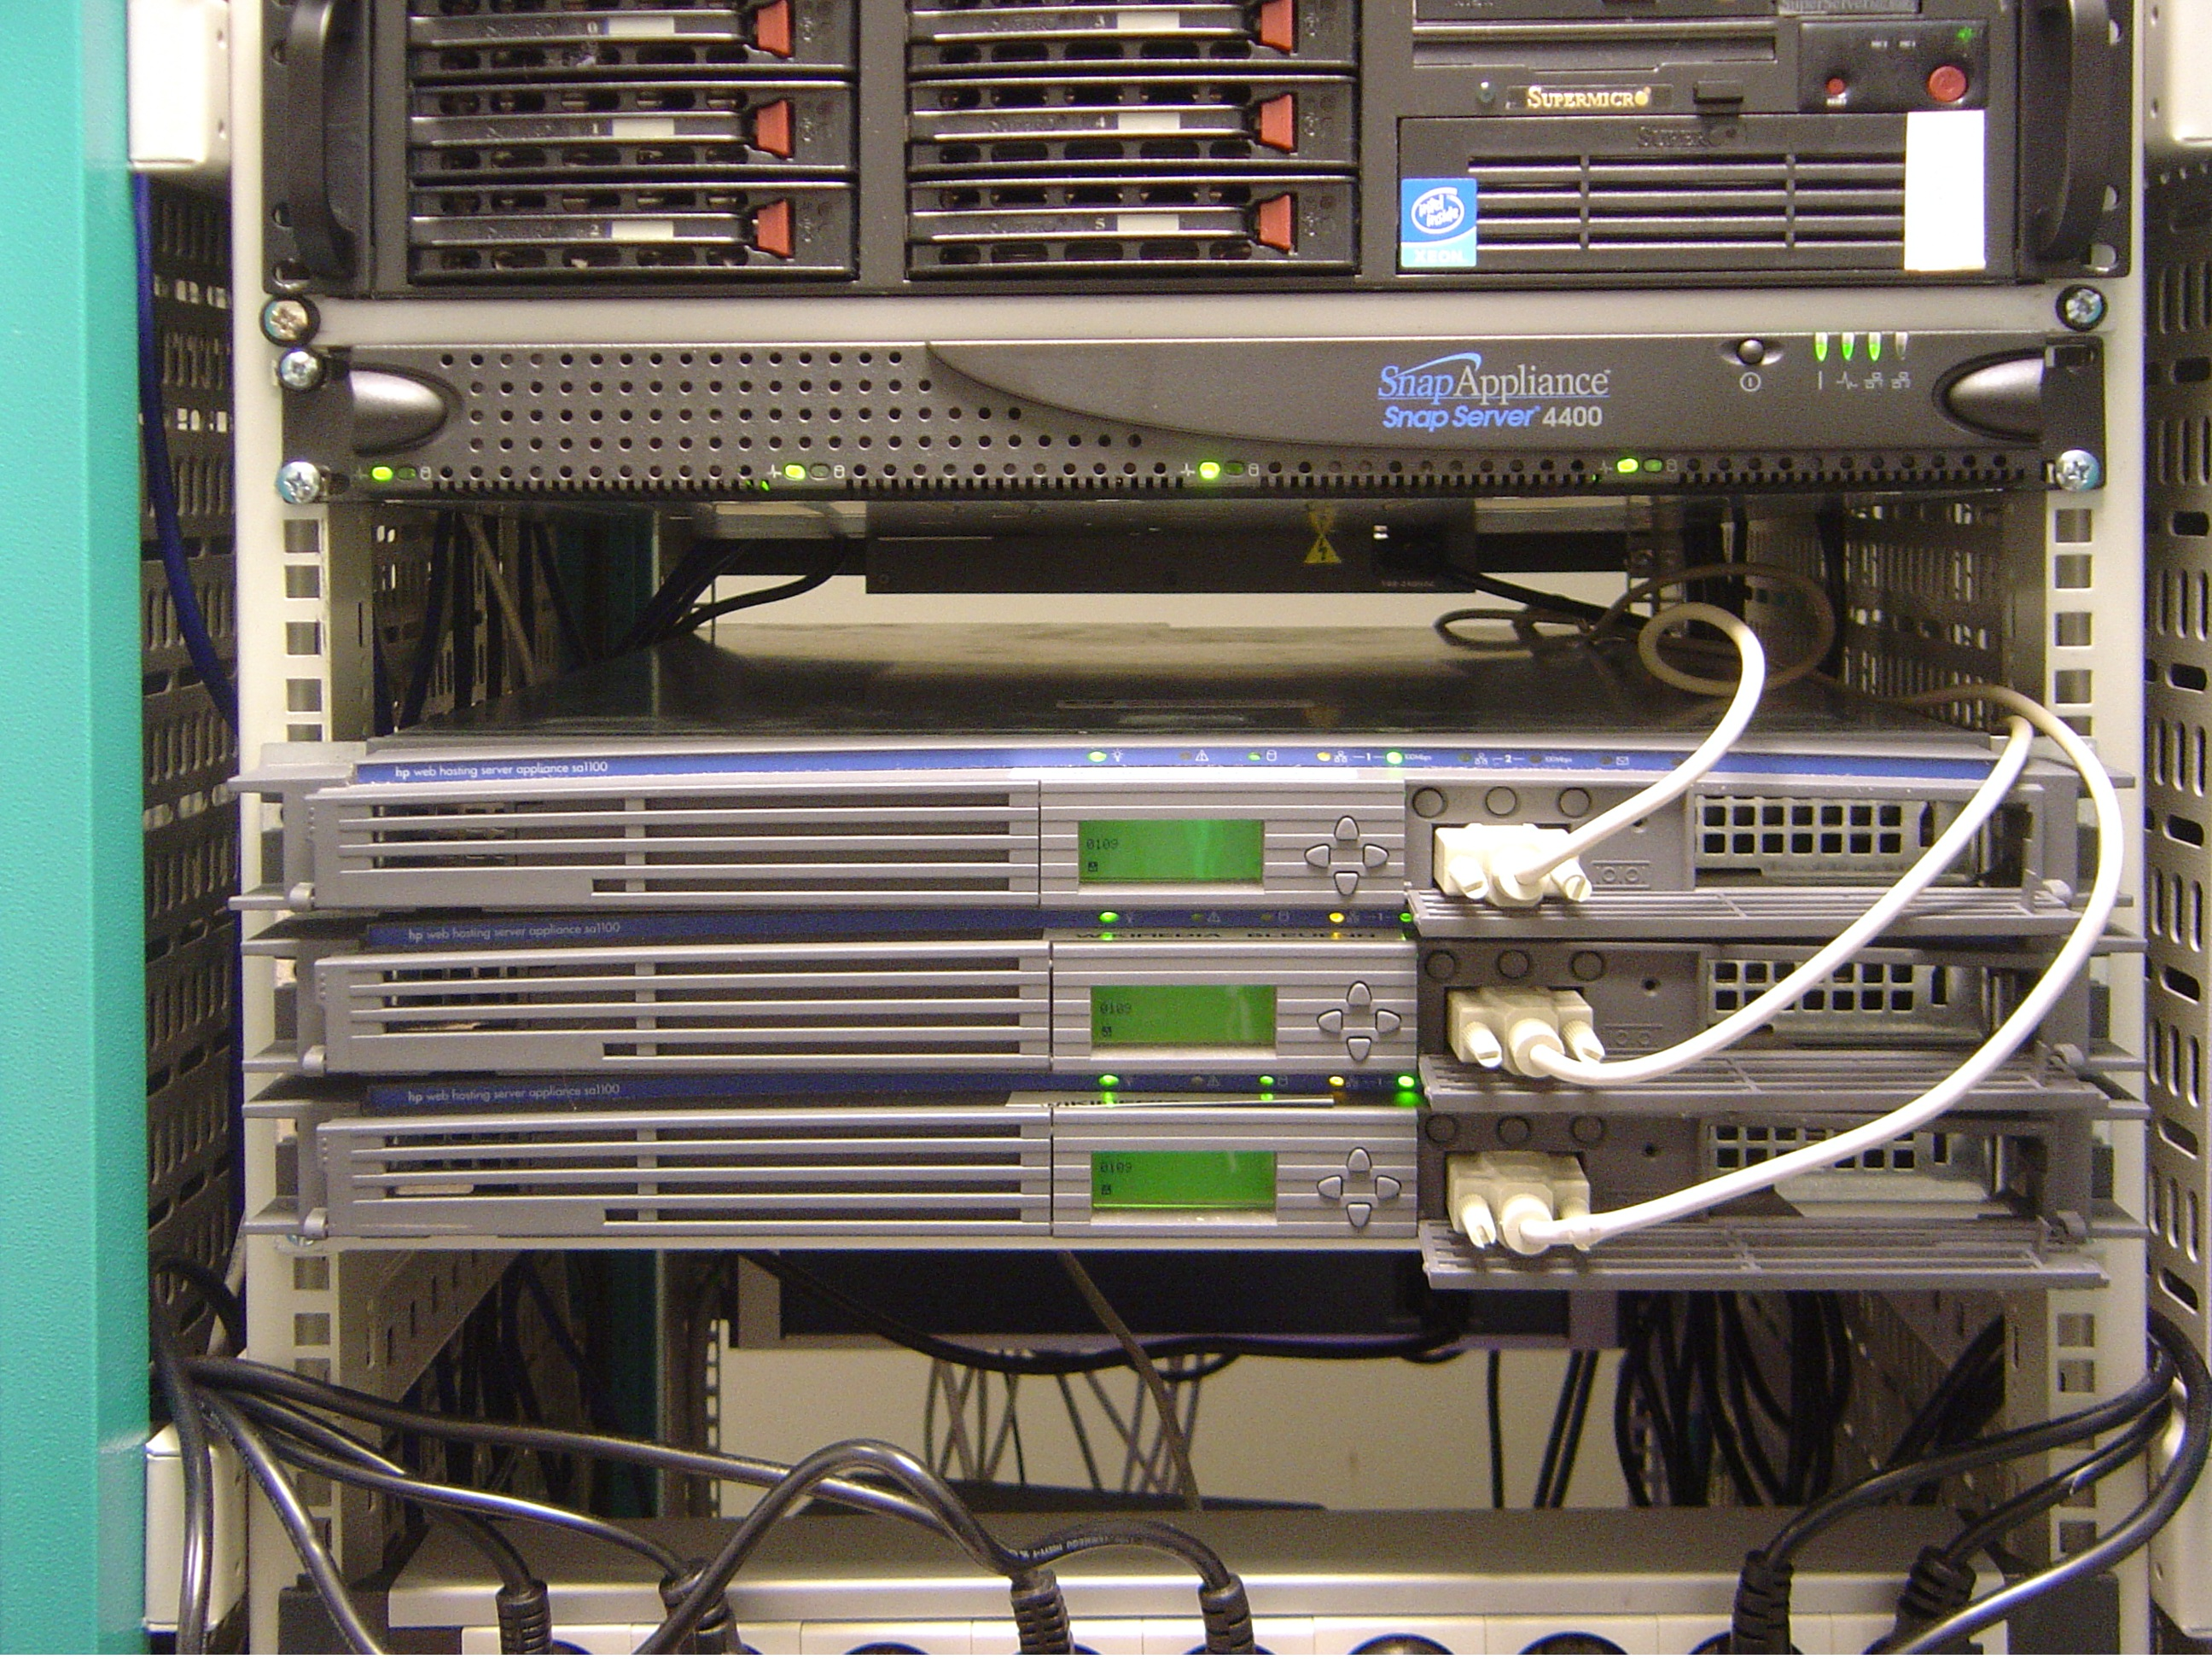
\includegraphics[width=0.5\textwidth]{base/Introduction/Case_wikipedia.jpg}
 \caption{Корпуса серверов Википедии}
 \label{base:introduction:components:case:wikipediacasepic}
\end{figure}
Внутреннее пространство поделено на несколько секций: отсек под устройства формата 5,25 дюймов, отсек под устройства формата 3,5 дюйма, место крепления блока питания и место для крепления материнской платы.

Корпуса могут быть разных форм и размеров. Относительно пропорций есть два устоявшихся форм-фактора: горизонтальные и вертикальные. Среди горизонтальных форм-факторов можно отметить:
\begin{description}
 \item[Desktop] $533\times419\times152$\,мм
 \item[FootPrint] $406\times406\times152$\,мм
 \item[SlimLine] $406\times406\times101$\,мм
 \item[UltraSlimLine] $381\times352\times75$\,мм
\end{description}
Также к горизонтальным форм-факторам можно причислить стоечные корпуса.

Вертикальные форм-факторы встречаются наиболее часто в офисах, домах, компьютерных классах. Они объеденены общим названием \emph{Tower} (minitower, miditower, bigtower). Среди причин их распространённости можно отметить больший объём по сравнению с горизонтальными, за счёт чего внутри остаётся больше места для вентиляции или дополнительных компонентов.

Вне зависимости от форм-фактора, системный блок является своеобразной <<печкой>>. Для охлаждения устройств, расположенных в нём, используется система вентиляции или циркуляции охлаждённой жидкости. Вентиляцию обеспечивают специальные вентиляторы (\emph{кулеры}, англ. \emph{cooler}), расположенные как на наиболее тепловыделяющих уст\-ройствах, так и на самом корпусе.
Довольно часто кулеры ставятся парно и однонаправлено, таким образом получается, что один задумает воздух внутрь, а другой выдувает наружу. За счёт этого обеспечивается постоянный поток воздуха, который оказывает охлаждающее действие.
Также кулеры устанавливают на одну из боковых стенок вертикальных форм-факторов, и иногда на вертикальные. Т.\,к.~охлаждение --- необходимый для нормального функционирования компьютера процесс, к его осуществлению надо подходить очень внимательно.
В частности, представляется недопустимым помещение системных блоков в тестные ниши современных компьютерных столов, т.\,к.~ограниченность пространства этих ниш делает задачу охлаждения труднорешаемой, а установленные средства воздушного охлаждения --- малоэффективными.

\subsubsection{Центральный процессор}\label{base:introduction:components:cpu}
Теперь рассмотрим \emph{центральный процессор} --- главное управляющее устройство, исполняющее машинные инструкции.
Изначально термин центральное процессорное устройство описывал специализированный класс логических машин, предназначенных для выполнения сложных компьютерных программ.
Вследствие довольно точного соответствия этого назначения функциям существовавших в то время компьютерных процессоров, он естественным образом был перенесён на сами компьютеры.
Начало применения термина и его аббревиатуры по отношению к компьютерным системам было положено в 1960-е годы.
Устройство, архитектура и реализация процессоров с тех пор неоднократно менялись, однако их основные исполняемые функции остались теми же, что и прежде.

\begin{figure}[h!]
 \centering
 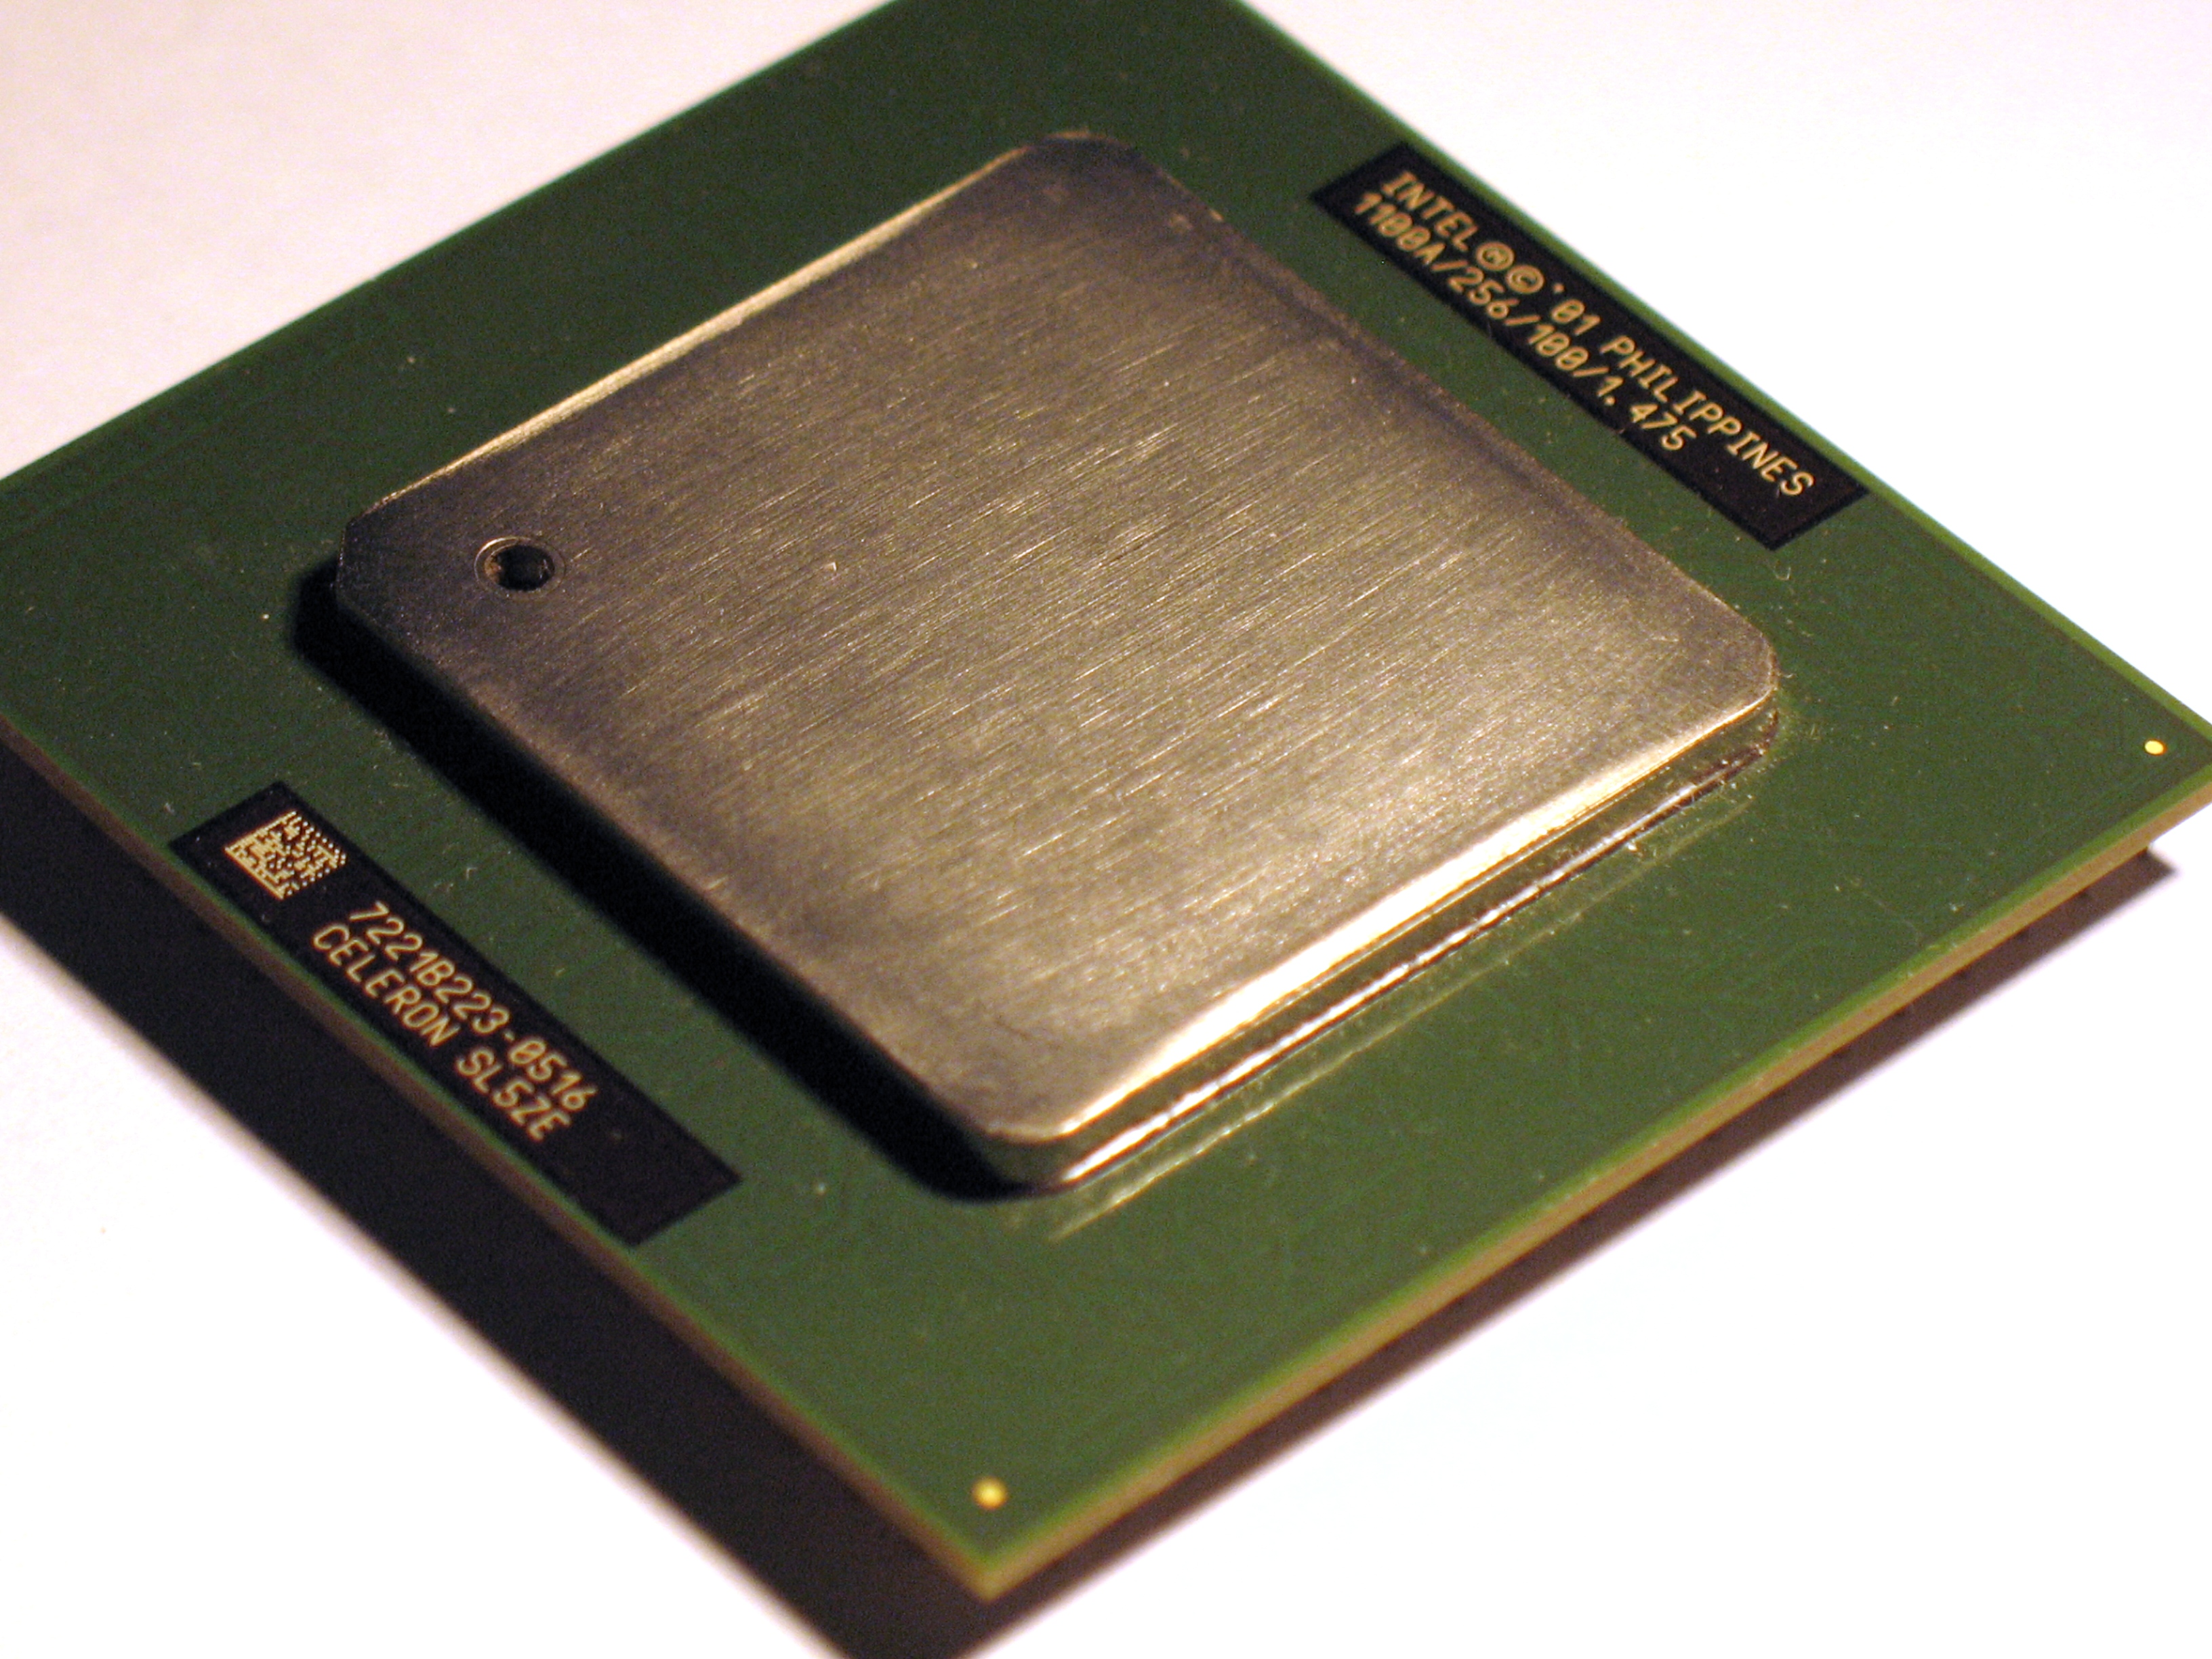
\includegraphics[width=0.33\textwidth]{base/Introduction/CPUup.jpg}
 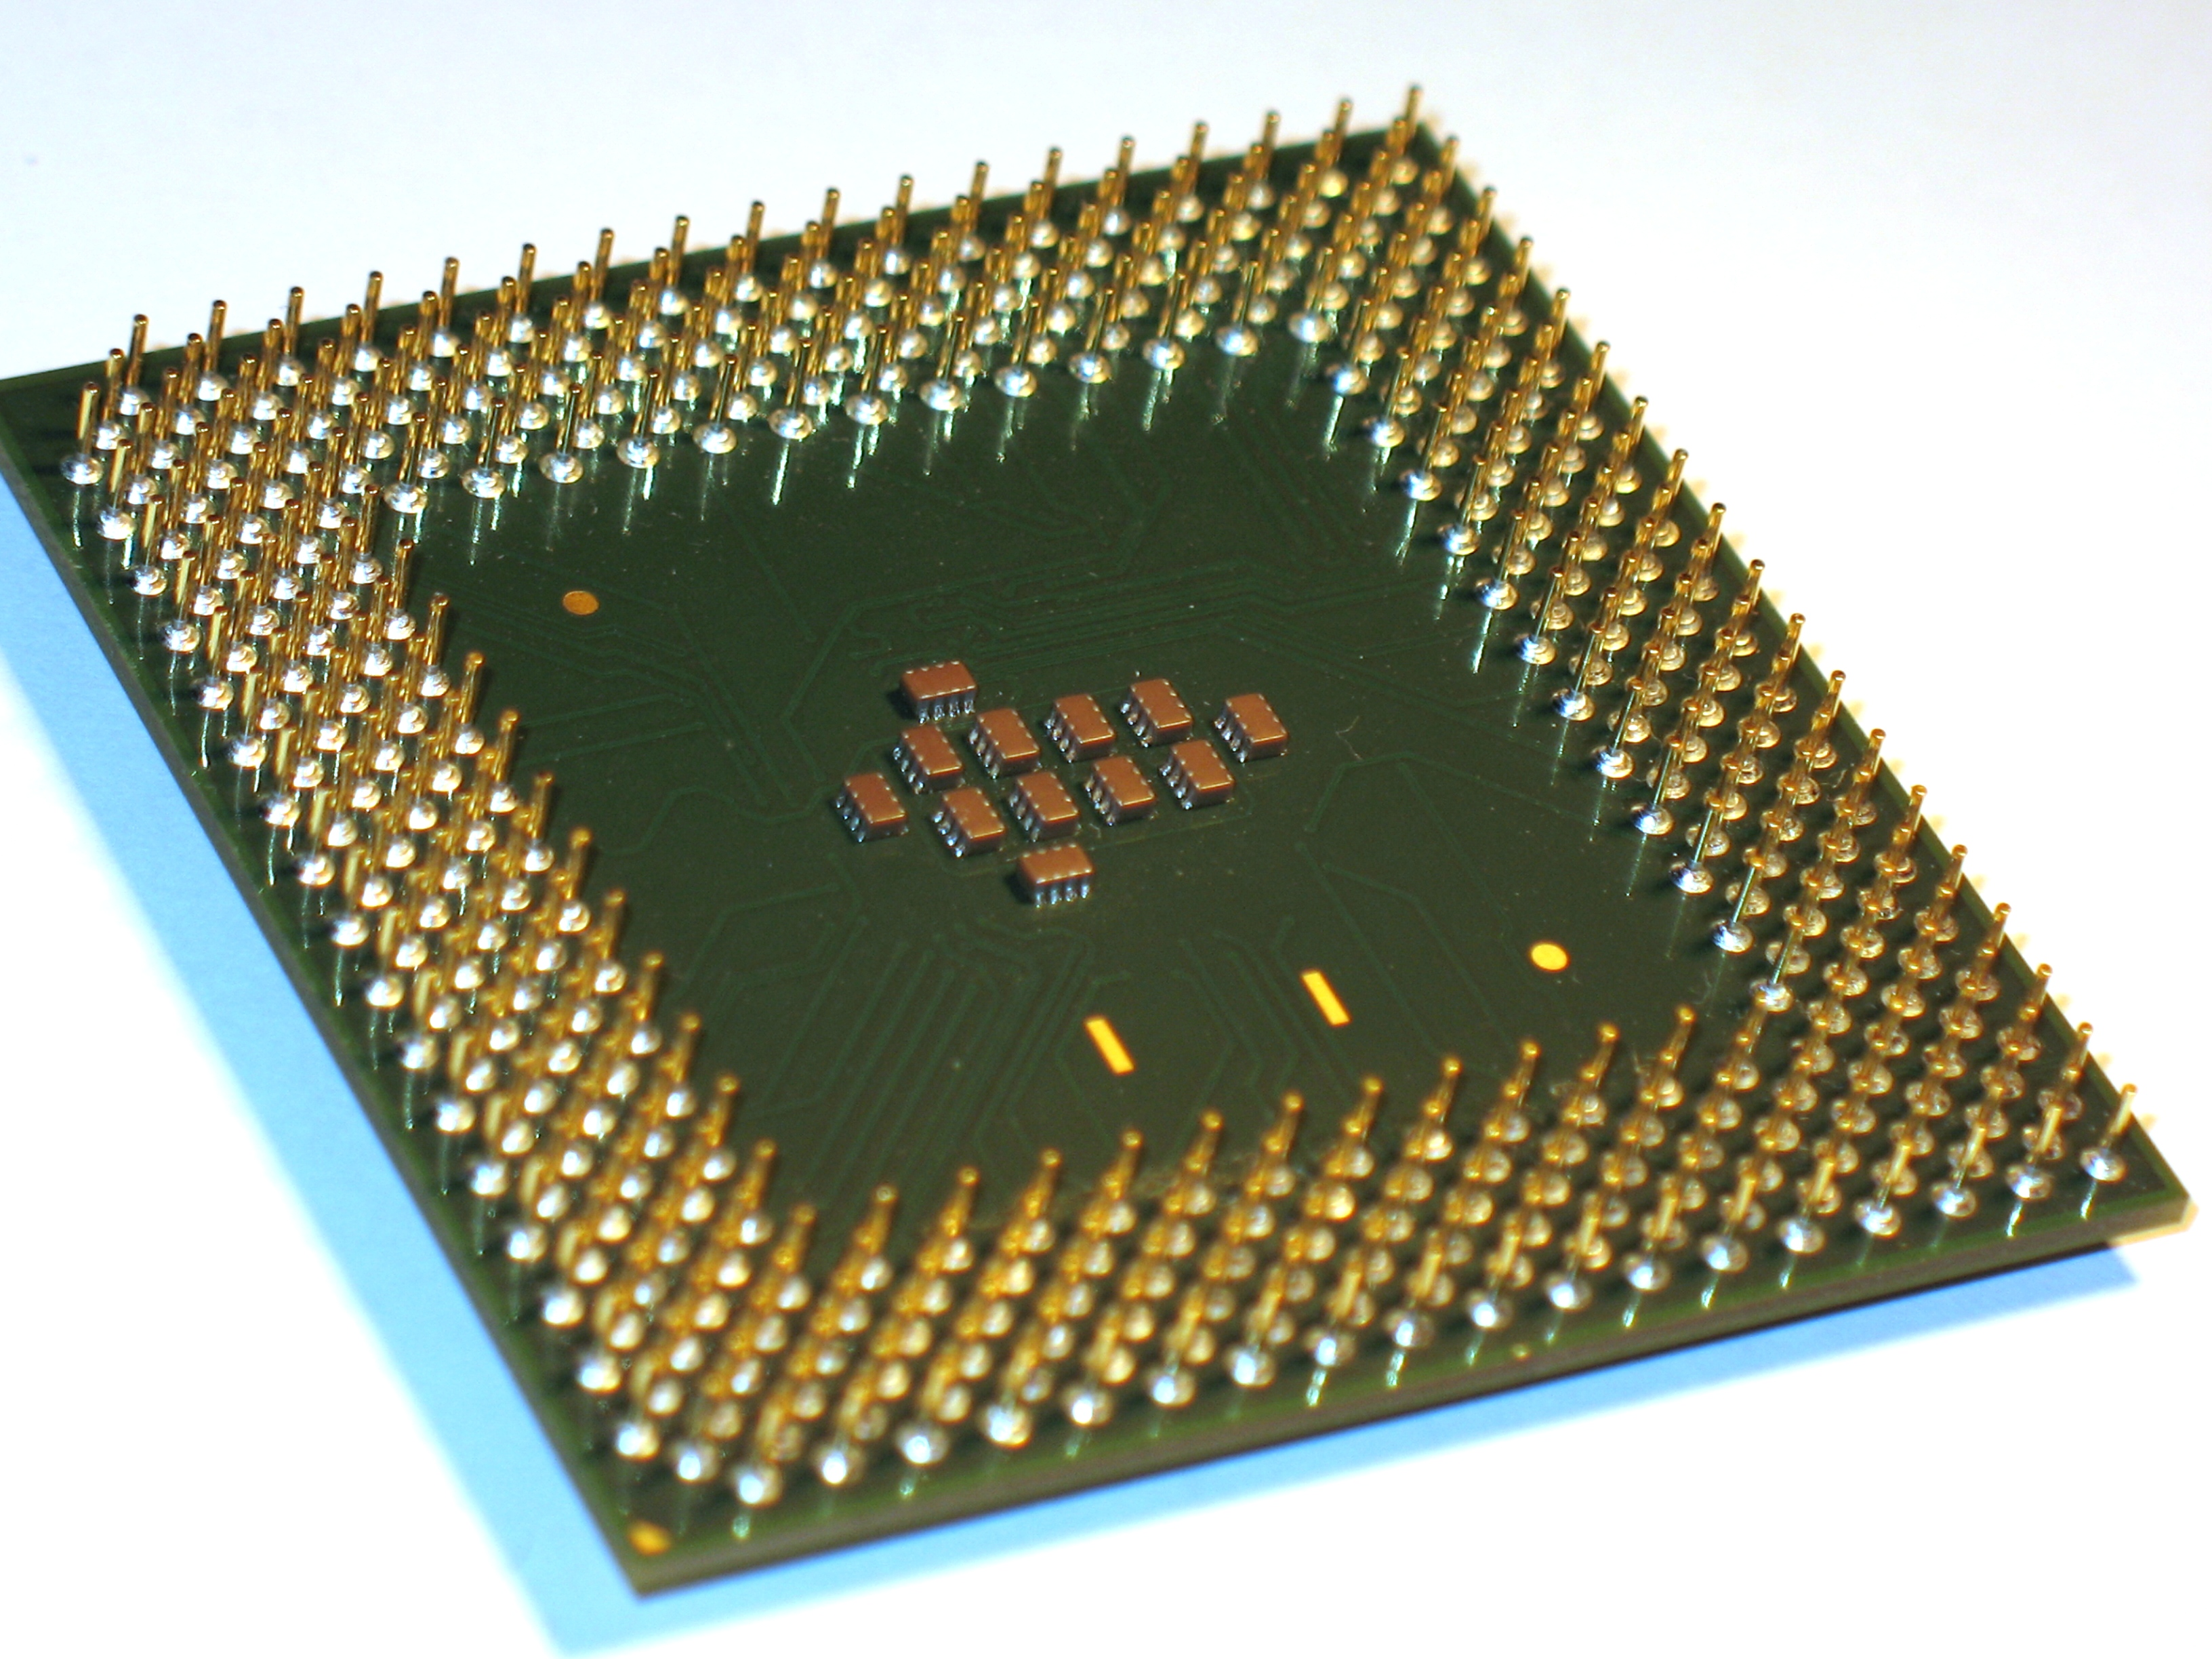
\includegraphics[width=0.33\textwidth]{base/Introduction/CPUdown.jpg}
 \label{base:introduction:components:cpu:cpupic}
 \caption{Центральный процессор}
\end{figure}

Главными характеристиками ЦПУ являются: \emph{тактовая частота}, \emph{производительность}, \emph{энергопотребление}, \emph{архитектура} и \emph{нормы литографического производственного процесса}. Рассмотрим их поподробнее:

\textbf{Производительность} --- это количественная характеристика скорости выполнения определённых операций на компьютере.
Чаще всего вычислительная мощность измеряется во флопсах (количество операций с плавающей запятой в секунду), а также производными от неё.
На данный момент принято причислять к суперкомпьютерам системы с вычислительной мощностью более 10 Терафлопс ($10\times10^{12}$ или десять триллионов флопс; для сравнения среднестатистический современный настольный компьютер имеет производительность порядка 0,1 Терафлопс).

Существует несколько сложностей при определении вычислительной мощности компьютера.
Во-первых, следует иметь в виду, что производительность системы может сильно зависеть от типа выполняемой задачи.
В частности, отрицательно сказывается на вычислительной мощности необходимость частого обмена данных между составляющими компьютерной системы, а также частое обращение к памяти.
В связи с этим выделяют пиковую вычислительную мощность --- гипотетически максимально возможное количество операций над числами с плавающей запятой в секунду, которое способен произвести данный компьютер.

\textbf{Тактовая частота} --- как следует из названия, определяет количество тактов, выполняемых за секунду. Условно можно переопределить это понятие как <<количество инструкций в секунду>>.
Среди потребителей имеется распространённое заблуждение о том, что процессоры с более высокой тактовой частотой всегда имеют более высокую производительность, чем процессоры с более низкой тактовой частотой.
На самом деле это не совсем так, т.\,к.~за один такт на разных процессорах может выполняться разное количество инструкций.

\textbf{Норма литографического процесса} --- описание технического процесса при производстве процессора. Наиболее важной характеристикой является разрешающая способность оборудования --- то есть, как следствие, плотность нанесения элементов.

\textbf{Архитектура} процессора --- количественная составляющая компонентов микроархитектуры процессора компьютера (например, регистр флагов или регистры процессора), рассматриваемая IT-специалистами в аспекте прикладной деятельности.
С точки зрения программиста --- совместимость с определённым набором команд, их структуры и способа исполнения.
С точки зрения аппаратной составляющей вычислительной системы --- это некий набор свойств и качеств, присущий целому семейству процессоров.
Имеются различные классификации архитектур процессоров, как по организации (например, по количеству и скорости выполнения команд: RISC, CISC), так и по назначению (например, специализированные графические).

\subsubsection{Оперативная память}\label{base:introduction:components:ram}
\begin{figure}[h!]
 \centering
 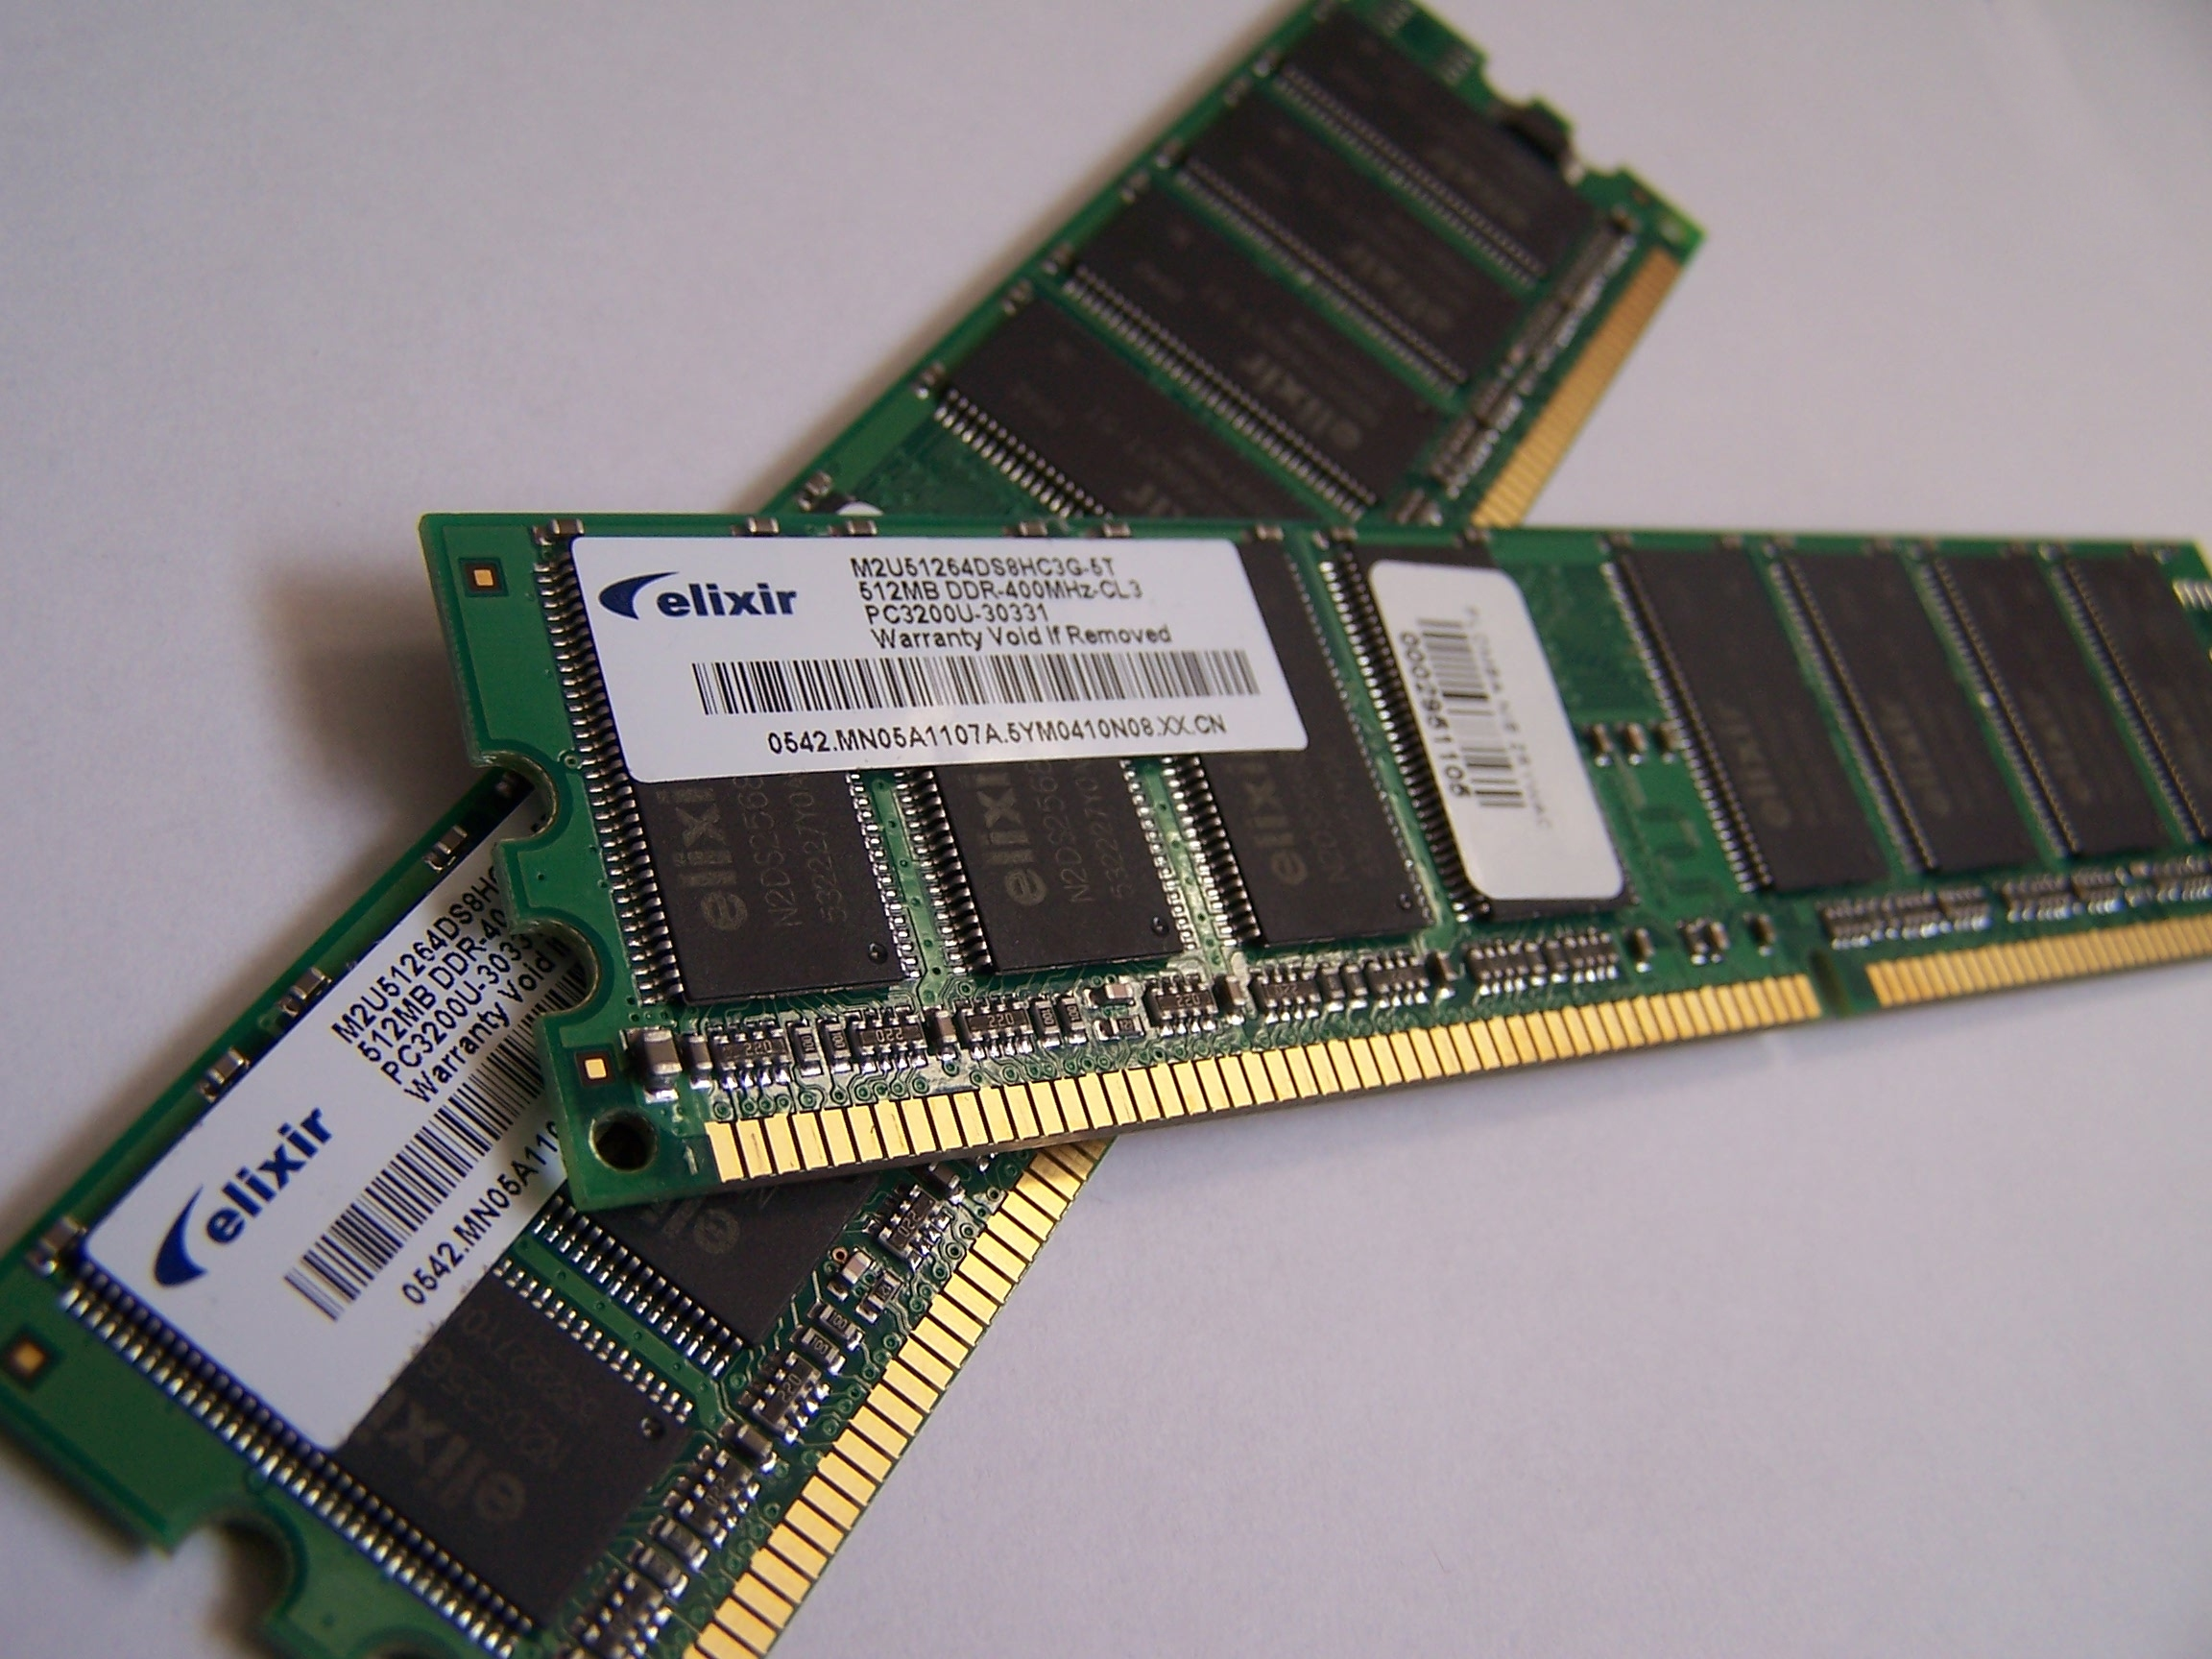
\includegraphics[width=0.5\textwidth]{base/Introduction/Memory.jpg}
 \label{base:introduction:components:ram:rampic}
 \caption{Плашки памяти DDRAM}
\end{figure}
\emph{Оперативно запоминающее устройство} --- энергозависимая плата, обеспечивающая временное хранение данных. Также часто синонимом ОЗУ выступает словосочетание <<\emph{оперативная память}>> --- по сути, его основная функция.
В оперативной памяти хранятся данные приложений, операционная система и многое другое.
Именно отсюда центральный процессор берёт инструкции для выполнения, записанные в программе, и именно сюда записывает их результат.
Даже если надо вывести простую строчку текста на экран, эта строчка будет размещена в оперативной памяти, и лишь затем будет считана оттуда для вывода.
Как следствие, к ней идёт постоянное обращение и происходит постоянный обмен данными.
За счёт этого растут требования к скорости памяти, отчего она получила своё название, а вместе с этим и стоимость.
Оперативная память стоит очень дорого (250--1875~руб. за гигабайт у ОЗУ при 1,5--3,75~руб. за гигабайт у жёстких дисков), притом что её использует каждое приложение для хранения данных.

Основными параметрами оперативной памяти являются \emph{объём} и \emph{частота шины}.
В качестве объёма указывается количество данных, которое может быть помещено в память.
Частота шины же показывает, сколько операций может быть совершено за еденицу времени, таким образом плата с большей частотой окажется быстрее платы аналогичного объёма, но с реже обновляемой шиной.
Стоит отметить, что на памяти указывается \emph{максимальная} частота, а не фактическая.
Реальная скорость также зависит от частоты шины на материнской плате, и из двух будет использоваться самая медленная.

У других устройств могут быть свои аналоги оперативной памяти, призванные снизить нагрузку на оную и/или ускорить получение данных.
Например, в процессорах, особенно в центральном, имеется \emph{кеш-память}, обладающая огромной скоростью даже по сравнению с оперативной, куда записываются самые частоиспользуемые инструкции или другие данные, вероятность обращения к которым крайне высока.
Аналогичные по функциям кеши имеют и некоторые другие устройства.
Объём их, как правило, очень мал, что не позволяет использовать их для ускорения работы системы

\subsubsection{Материнская плата}\label{base:introduction:components:motherboard}
\begin{figure}[h!]
 \centering
 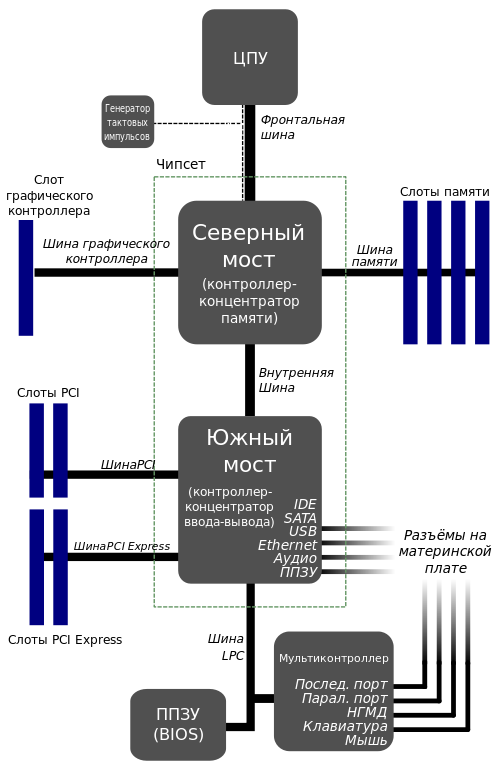
\includegraphics[width=0.9\textwidth]{base/Introduction/Motherboard_diagram.png}
 \caption{Схема устройства материнской платы}
 \label{base:introduction:components:motherboard:diagrampic}
\end{figure}
\begin{figure}
 \centering
 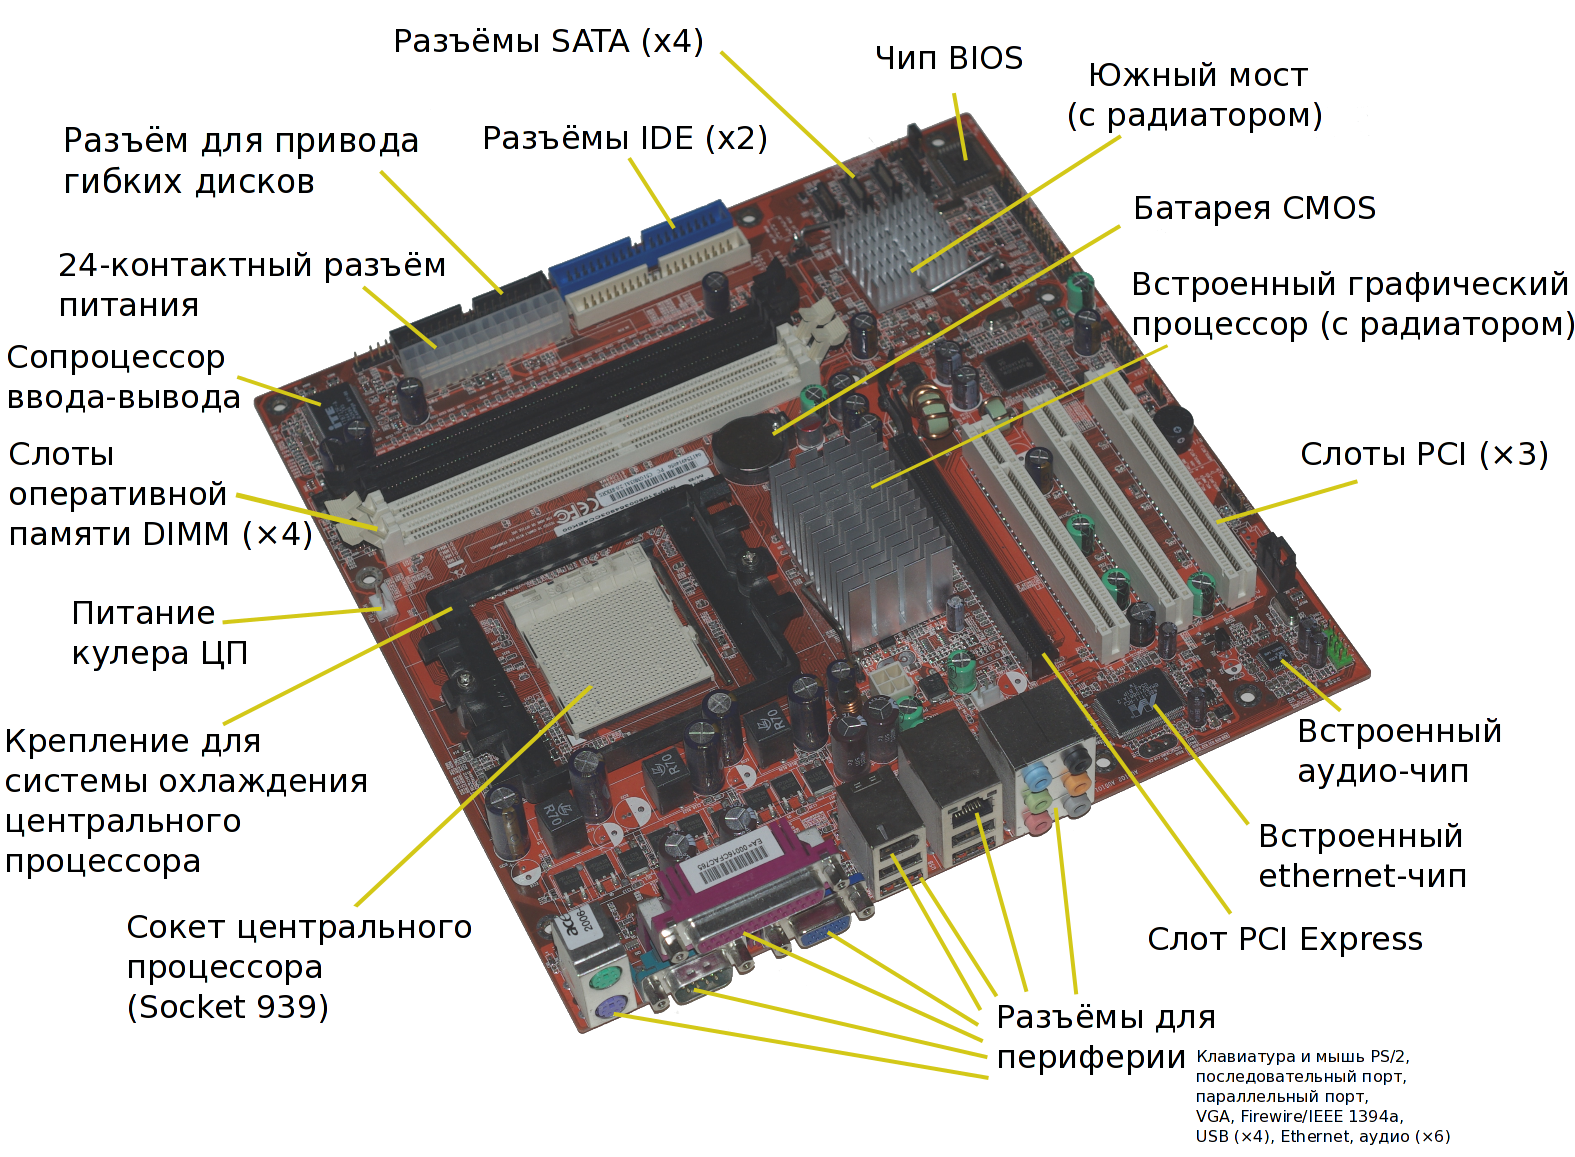
\includegraphics[width=\textwidth]{base/Introduction/Motherboard.png}
 \label{base:introduction:components:motherboard:motherboardpic}
\end{figure}
Следующей рассмотрим основную плату компьютера, соединяющую всё воедино.
\emph{Материнская плата} (англ. \emph{motherboard}, \emph{MB}) --- сложная многослойная печатная плата, на которой устанавливаются основные компоненты персонального компьютера.
Именно материнская плата объединяет и координирует работу таких различных по своей сути и функциональности комплектующих, как процессор, оперативная память, платы расширения и всевозможные накопители.

Современные материнские платы содержат, как минимум:
\begin{itemize}
 \item сокет для ЦПУ;
 \item слоты для оперативной памяти;
 \item \emph{чипсет} (англ. \emph{chipset}), являющийся основным средством взаимодействия между устойствами;
 \item энергонезависимую память, хранящую BIOS и прочее необходимое ПО;
 \item тактовый генератор, используемый для синхронизации различных компонентов;
 \item слоты расширения;
 \item разъёмы для подключения внешнего источника питания, а также разъёмы для обеспечения питанием некоторых устройств (например, кулер ЦПУ).
\end{itemize}

Также, почти все материнские платы включают логику и разъёмы для поддержки часто используемых устройств ввода, таких как PS/2 для подключения мыши и клавиатуры.
Иногда они могут содержать графические интерфейсы и простые графические процессоры.
Дополнительная периферия, такая как дисковые контроллеры, может быть представлена платами расширения.

Учитывая большое тепловыделение быстрых процессоров и прочих устройств, современные материнские платы имеют радиаторы и точки для крепления дополнительных вентиляторов.

Чипсет --- это набор системной логики, набор микросхем, обеспечивающих подключение ЦПУ к ОЗУ и контроллерам периферийных устройств.
Как правило, современные наборы системной логики строятся на базе двух схем: <<северного>> и <<южного мостов>>.

\emph{Северный мост} (англ. \emph{Northbridge}), \emph{MCH} (\emph{Memory controller hub}), \emph{системный контроллер} --- обеспечивает подключение ЦПУ к узлам, использующим высокопроизводительные шины: ОЗУ, графический контроллер.
Обычно к системному контроллеру подключается ОЗУ, в этом случае он содержит в себе контроллер памяти.
Таким образом, от типа применённого системного контроллера обычно зависит максимальный объём ОЗУ, а также пропускная способность шины памяти персонального компьютера.
Однако в настоящее время имеется тенденция встраивания контроллера ОЗУ непосредственно в центральный процессор, что упрощает функции системного контроллера и снижает тепловыделение.
В качестве шины для подключения графического контроллера на современных материнских платах используется PCI Express.
Ранее использовались общие шины (ISA, VLB, PCI) и шина AGP.

\emph{Южный мост} (англ. \emph{Southbridge}), \emph{ICH} (\emph{I/O controller hub}), \emph{периферийный контроллер} --- содержит контроллеры периферийных устройств (таких как жёсткого диска, Ethernet, аудио), контроллеры шин для подключения периферийных устройств (шины PCI, PCI Express и USB), а также контроллеры шин, к которым подключаются устройства, не требующие высокой пропускной способности.

\subsubsection{Видеокарта}\label{base:introduction:components:videocard}


\subsubsection{Звуковая карта}\label{base:introduction:components:soundcard}


\subsubsection{Сетевая карта}\label{base:introduction:components:nic}


\subsubsection{Блок питания}\label{base:introduction:components:psu}


\subsection{Монитор}\label{base:introduction:components:monitor}


\subsection{Периферия}\label{base:introduction:components:peripheral}


\subsection{Принтеры, сканеры и МФУ}\label{base:introduction:components:printers}

